\begin{figure}
\hspace*{-6mm}
\begin{tikzpicture}
  \node[font=\itshape] (textA) {\(\forall g\in\{Z,S,T\}\) at control wire};
  \node [below=-5mm of textA] (A) {
    \begin{tikzpicture}
      \node[inner sep=0pt] (c1) at (0,0) {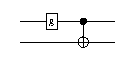
\includegraphics[scale=2]{Figures/circuits/C_gCNOT}};       
      \node[right=-13.9mm of c1.east, inner sep=0pt] (c2) {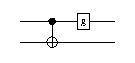
\includegraphics[scale=2]{Figures/circuits/C_CNOTg}};
      \node[right=-12mm of c1.east, rectangle, fill=white, minimum size=10mm] (eq) {\(=\)};  
      \node[right=7mm of c1.west, rectangle,fill=white,minimum width=5mm, minimum height=10mm] {};
      \node[left=7mm of c2.east, rectangle,fill=white,minimum width=5mm, minimum height=10mm] {};
    \end{tikzpicture}
  };
  \node[right=20mm of textA, font=\itshape] (textB) {\(\forall g\!\text{'}\in\{X,Y\}\) at control wire};
  \node [below=-5mm of textB] (B) {
    \begin{tikzpicture}
      \node[inner sep=0pt] (c1) at (0,0) {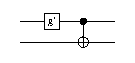
\includegraphics[scale=2]{Figures/circuits/C_g2CNOT}};       
      \node[right=-13.9mm of c1.east, inner sep=0pt] (c2) {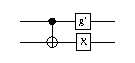
\includegraphics[scale=2]{Figures/circuits/C_CNOTg2}};
      \node[right=-12mm of c1.east, rectangle, fill=white, minimum size=10mm] (eq) {\(=\)};  
      \node[right=7mm of c1.west, rectangle,fill=white,minimum width=5mm, minimum height=10mm] {};
      \node[left=7mm of c2.east, rectangle,fill=white,minimum width=5mm, minimum height=10mm] {};
    \end{tikzpicture}
  };
  \node[below=20mm of textA, font=\itshape] (textC) {\(\forall g\in\{X\}\) at target wire};
  \node [below=-5mm of textC] (C) {
    \begin{tikzpicture}
      \node[inner sep=0pt] (c1) at (0,0) {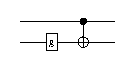
\includegraphics[scale=2]{Figures/circuits/T_gCNOT}};       
      \node[right=-13.9mm of c1.east, inner sep=0pt] (c2) {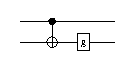
\includegraphics[scale=2]{Figures/circuits/T_CNOTg}};
      \node[right=-12mm of c1.east, rectangle, fill=white, minimum size=10mm] (eq) {\(=\)};  
      \node[right=7mm of c1.west, rectangle,fill=white,minimum width=5mm, minimum height=10mm] {};
      \node[left=7mm of c2.east, rectangle,fill=white,minimum width=5mm, minimum height=10mm] {};
    \end{tikzpicture}
  };
  \node[below=20mm of textB, font=\itshape] (textD) {\(\forall g\!\text{'}\in\{Y,Z\}\) at target wire};
  \node [below=-5mm of textD] (D) {
    \begin{tikzpicture}
      \node[inner sep=0pt] (c1) at (0,0) {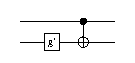
\includegraphics[scale=2]{Figures/circuits/T_g2CNOT}};       
      \node[right=-13.9mm of c1.east, inner sep=0pt] (c2) {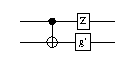
\includegraphics[scale=2]{Figures/circuits/T_CNOTg2}};
      \node[right=-12mm of c1.east, rectangle, fill=white, minimum size=10mm] (eq) {\(=\)};  
      \node[right=7mm of c1.west, rectangle,fill=white,minimum width=5mm, minimum height=10mm] {};
      \node[left=7mm of c2.east, rectangle,fill=white,minimum width=5mm, minimum height=10mm] {};
    \end{tikzpicture}
  };
\end{tikzpicture}
\caption{Different cases when a 1-qubit gate from Clifford+$T$ can be pushed through a CNOT gate.}
\label{fig:pullRules}
\end{figure}